\chapter{Background}\label{chap:bkgnd}
%
\begin{epigraphs}
  \qitem{...mere metrical measurement is not \gls{tala}. It is a harmonious correlation of discipline and freedom.}{\citeA[p. 61]{shankar:99:music}, from \textit{The art and science of carnatic music}, Parampara Publications.}
  %\qitem{More text \ldots}
  %{\emph{That story}. \\ Short story by that guy}
\end{epigraphs}
% Use \noindent for the first paragraph after this
%
%\note{Background: Music and the state of the art}
%\note{\textit{Chapter in brief: Provide a concrete terminology with rhythm terms, and a just sufficient music background in CM, HM, MMT, BO. Provide a detailed discussion and review of the state of the art in rhythm analysis, stressing mainly on the tasks of onset detection, tempo estimation, beat and downbeat tracking, percussion pattern transcription and discovery. If needed, provide some technical background.  The material in the chapter is mainly derived out of JNMR (2014), books and literature review.}}
% We focus on the rhythmic aspects of Hindustani and Carnatic music. The concept of tāla forms the central theme in rhythm modeling of Indian music. The main rhythmic accompaniment in Hindustani music is the Tabla, while its Carnatic counterpart is the \emph{Mridangam (Mr̥daṅgaṁ)}. We first provide an introduction to rhythm in these two music traditions. We then survey the related work in this area of research and discuss the state of the art. 
\noindent The chapter provides the necessary music and technical background for understanding the work presented in the dissertation. The main aims of this chapter are:
\begin{enumerate}[leftmargin=*,itemsep=0pt]
  \item To establish a consistent terminology for several rhythm related music concepts
  \item To describe relevant rhythm related concepts in Indian art music and Beijing opera 
  \item To present an overview of the state of the art for the automatic rhythm analysis problems addressed in the dissertation
	\item To briefly describe the technical concepts necessary to understand the algorithms and methods presented in the dissertation
\end{enumerate}
\section{Rhythm: terminology}
As observed already many decades ago, discussions about rhythm tend to suffer from inconsistencies in their terminology \cite{sachs:53:rhythm}. Let us therefore try to locate definitions for some basic terms, in order to establish a consistent representation in the dissertation. Gy\"orgy Ligeti, a European composer who showed a high interest in rhythmic structures in music of African cultures, defined rhythm as ``every temporal sequence of notes, sounds and musical \textit{Gestalten}", while he referred to meter\index{Meter} as ``a more or less regular structuring of temporal development" \cite{ligeti:07:schriften}. According to that definition, rhythm is contained in all kinds of music, while pulsating rhythm which is subordinated to a meter is not found in all music. \citeA{kolinski:73:rhythm} describes the regular structuring caused by meter as organized pulsation, which functions as a framework for rhythmic design. 

Pulsations in meter are organized into hierarchical levels of differing time spans, usually demanding the presence of pulsation at least on three levels; these levels are referred to as subdivision (also called the \textit{tatum}\index{Tatum}), beat (also called the \textit{tactus}\index{Tactus}), and measure (or bar): from short to long time-span \cite[accessed June 2016]{london:12:grovemeter}. The pulsation at the beat level was referred to as primary rhythmic level by \citeA{cooper:60:rhythm}, and they define it as the lowest level on which a complete rhythmic group is realized. The same authors identify this level with a subjective notion as well, by referring to it as the level at which the beats are felt and counted. As listeners tend to count the beats at varying levels \cite{parncutt:94:perception,muller:11:intro}, and what can be considered a complete rhythmic group can be argued as well, we are confronted with a significant amount of ambiguity in determining this level for a piece of music. Finding a clear terminology is further hampered by the fact that the pulsation at the beat level is commonly also referred to as ``beat" or ``pulse" as observed by \citeA{london:04:time}. A shortcoming of most attempts to describe rhythm and meter is the assumption about pulsation to consist of recurring, precisely equivalent and equally-spaced isochronous \index{Isochronicity} stimuli \cite{lerdahl:83:generative}. Such preconditions cause difficulties when analyzing music of other cultures since in many cases, mutual equidistance becomes an exception rather than the rule, taking the important role of additive meters in Indian, Greek and Turkish music as one example. 

In order to obtain a consistent terminology, we consider meter as being an organization of pulsation into different levels related to the time-spans of the individual pulsations. Note that this may include an irregular pattern of unequal time-spans at some level, e.g. due to the presence of an additive meter\index{Additive meter}. We will consider pulsations on three levels. On the (lower) subdivision level, we will refer to subdivision pulsation or subdivision pulses, depending on if we refer to the time series that constitutes the pulsation or to the individual instances of the pulsation, respectively. On the beat level, we will differentiate between the beat pulsation, and beats as its instances (instead of the inconvenient term of ``beat pulses"). On the bar level, the term pulsation is not appropriate due to the often larger time-span at this level. Therefore, we use the notions of bar length to describe the time-span at this level and downbeat as the beginning of a bar. The overall structure of a meter is defined by the time-span relations between these three levels. Typically, the time-span relation between bar and beat level is denoted as the bar length (in beats), and the relation between beat and subdivision level as the subdivision meter (in subdivision pulses). 

It was observed by e.g.~\citeA{clayton:00:time} that meter in music causes a transformation of time from linear development to a repetitive and cyclic structure. This happens because its levels of pulsation constitute what we want to refer as metrical cycles. Throughout the text, we put emphasis on terms containing the notion of a cycle (such as the measure cycle for the cycle repeating on every downbeat), a notion suitable in the musical context of Indian art music. In addition, in Indian art music, the beats or the subdivisions of a bar can be grouped to form musically defined metrical structures, broadly called sections of the bar. The metrical structures in Indian music are discussed next, with an introduction to the Indian art music traditions of Hindustani and Carnatic music.
%\note{Definitions and descriptions of meter, rhythm, pattern, pulsation as defined in state of the art.}
%\dtext{Describe and define rhythm, provide several views. Discuss several definitions provided in theory, Talk about inconsistency in rhythm terminology. Define pulse, define universals in rhythm with references. Rhythm is organized in several levels: tatum, tactus, meter. Defining tempo. The problem of defining beats and cycles - non-isochronous beats. Perceptual present, and its influence - cyclic and additive meters, long cycles, and how we define them.}
%\dtext{Percussion patterns, how they are defined.}
\section{Music background}\label{sec:musicbkgnd}
%\comment{The bare minimum needed to understand the thesis.}
%\dtext{Here we talk about music cultures and associated concepts around them that are useful to the problems. This is not a comprehensive treatment of the subject and more is in the references cited.}
This section describes the primary music cultures that are the focus of study in this dissertation. The focus is on rhythm and percussion related concepts in these music cultures. This section is not a comprehensive treatment of the subject, and is just sufficient to follow the rest of the chapters of the dissertation. Hence, additional references that contain an in-depth discussion of the presented concepts are provided when necessary. 
\subsection{Indian art music}
%\dtext{Indian Art music is Carnatic and Hindustani music. No of listeners they have and what is the basic idea in their sound texture, characteristics, oral traditions, have significant musicology. Why did we choose them, and how they can be studied. Some resources at a broad level.}
% One paragraph on Indian art music, and its context in the society
Hindustani (Hindustāni)\index{Hindustani music} and Carnatic (Karṇāṭaka)\index{Carnatic music} music are two of the most predominant art music traditions in India. Hindustani music is spread mainly over the northern parts of the Indian subcontinent (northern and central parts of India, Pakistan, Nepal, and Bangladesh), which is a huge geographic area with diverse cultures that influence the music. Carnatic music is predominant mainly in southern parts of the Indian subcontinent (South India and Sri Lanka). Both these musics have a long history of performance and continue to exist and evolve in the current sociocultural contexts. Both of them have a large audience and significant musicological literature that can used to formalize \gls{MIR} problems for these musics. The presence of a large dedicated audience and a significant musicological literature are a good motivation to study these music cultures from a computational perspective and build tools and methods for automatic melody and rhythm analysis in these music cultures. 

While the two musics differ in performance practices, they share similar melodic and rhythmic concepts. The melodic framework is based on \gls{raag} in Hindustani music and \gls{raga} in Carnatic music. The rhythmic framework is based on cyclic metrical structures called the \gls{taal} in Hindustani music and \gls{tala} in Carnatic music. 

There are several unfamiliar terms that are introduced in this section and hence before presenting those terms, a note on disambiguating terminology is in order. The latin transliteration of the Indian art music terms are according to the ISO 15919 (Transliteration of Devanagari and related Indic scripts into Latin characters) standard \cite{iso:01:15919trans}. Both the words \gls{taal} and \gls{tala} are Sanskritic in origin and have the same literal meaning of a ``hand-clap". The difference apparent in transliteration is due to their usage in Hindustani and Carnatic music. We use the language Hindi for all the terms of Hindustani music, and the South Indian language Kannada for all the terms of Carnatic music. Hence the latin transliteration of terms change accordingly. 

We will use the term Indian art music (or even Indian music) to refer collectively to Carnatic and Hindustani music. For consistency and convenience, when it is clear from the context, we will use the word \gls{tala} to mean both \gls{taal} and \gls{tala} when we refer collectively to the two Indian musics, and use the respective terms while referring to each music culture individually. 
% As mentioned earlier, the terms related to music related concepts use Kannada for Carnatic music terms and Hindi for Hindustani music terms.  For consistency, when it is clear from context, we use Carnatic music terminology to refer collectively to the two Indian art musics, e.g. we use the word \gls{tala} to mean both \gls{taal} and \gls{tala} when we refer collectively to the two Indian art musics. We use the respective terms while referring to each music culture individually. Further we will use the term Indian art music to refer collectively to Carnatic and Hindustani music.

In Carnatic music, a concert, called a \gls{kutcheri}, is the natural unit of Carnatic music and used as the main unit of music distribution. A concert has one or more lead artists - mainly vocal, vīṇā (commonly spelled veena), violin, or flute, melodic accompaniment (mainly violin), and one or more percussion accompaniments - mainly \gls{mridangam} (spelled commonly as mridangam). Carnatic music is predominantly composition based and most commercial releases are concerts, comprising of several pieces that are improvised renderings of compositions. Vocal music is predominant in Carnatic music and most of the compositions are composed to be sung. Even in instrumental music, the lead artist aims to mimic vocal singing, called the \textit{gāyaki} (singing) style \cite{vishwanathan:04:music}. The \gls{raga} and \gls{tala} are the most important metadata associated with a composition and hence a recording of the composition. Each composition is composed in one or more \glspl{raga} and \glspl{tala}. 

Due to the wider geographic extent of Hindustani music spread over the Indian subcontinent, it is diverse with several different music styles falling under its gamut. Several different styles of Hindustani music exist, but in the dissertation we focus mainly on \gls{khayal}, the most popular style of Hindustani music. 

A typical \gls{khayal} performance has lead vocals or a lead instrument (such as \gls{sitar}, \gls{sarod}, flute, \gls{santoor}), a melodic accompaniment (a harmonium or a \gls{sarangi}), and a percussion accompaniment \gls{tabla}. In \gls{dhrupad} style, \gls{pakhavaj} is the main percussion accompaniment. The artists in Hindustani music belong to what are called \glspl{gharana}, or stylistic schools. Though all the \gls{gharana} use the same music concepts and basic style, each of them have their own nuances that are well distinguished and documented \cite{mehta:08:gharana}. 

Rhythm in Indian art music revolves around the central theme of the \gls{tala} and hence it is the primary focus of this dissertation. Though the idea and purpose of a \gls{tala} in both music cultures is the same, there are significant fundamental differences in performance practices and terminology. An in-depth description of rhythm concepts in Indian art music is provided in the following section, highlighting these similarities and differences.
\subsection{Rhythm and percussion in Carnatic music}\label{sec:bkgnd:carRhythmIntro}
%\comment{In detail...}
% \dtext{How is rhythm organized. What is laya, tala. Different terms associated with the tala, and then some more terms. Average characteristic of rhythm - tempo ranges, hand gestures, angas (section/organs), nades, explain the figures. Mridangam and its role. Possibility of non-isochorous beats, but our definition of isochronous beats in the thesis and how we can get non-isochronous beats from isochronous ones later on.}
\citeA{samba:98:southMusic} provides a detailed description of \glspl{tala} in Carnatic music. In Carnatic music, the \gls{tala} provides a broad structure for repetition of music phrases, motifs and improvisations. It consists of fixed length time cycles called \gls{avartana} which can be referred to as the \gls{tala} cycle. In an \gls{avartana} of a \gls{tala}, phrase refrains, melodic and rhythmic changes occur usually at the beginning of the cycle. An \gls{avartana} is divided into basic equidistant time units called \glspl{akshara}. The first \gls{akshara} pulse of each \gls{avartana} is called the \gls{sama}, which marks the beginning of the cycle (or the end of the previous cycle, due to the cyclic nature of the \gls{tala}). The \gls{sama} is often accented, with notable melodic and percussive events. Each \gls{tala} also has a distinct, possibly non-regular division of the cycle period into sections called the \gls{anga}. The \glspl{anga} serve to indicate the current position in the \gls{avartana} and aid the musician to keep track of the movement through the \gls{tala} cycle. A movement through a \gls{tala} cycle is explicitly shown by the musician using hand gestures, based on the \glspl{anga} of the \gls{tala}. 

The common definition of an isochronous \index{Isochronicity} (equally spaced in time) beat pulsation, as the time instances where a human listener is likely to tap his/her foot to the music, is likely to cause problems in Carnatic music. Due the explicit hand gestures, listeners familiar to Carnatic music tend to tap to an non-isochronous sequence of beats in certain \glspl{tala}. Hence we use an adapted definition of a beat for the purpose of a common ground, defined as a uniform pulsation. It is to be noted however that an equidistant beat pulsation can later help in obtaining the musically relevant possibly irregular beat sequence that is a subset of the equidistant beat pulses. The \glspl{akshara} in an \gls{avartana} are grouped into equal length units, which we will refer to as the beats of the \gls{tala}. The perceptually relevant hand/foot tapping time ``beats" are a subset of this uniform beat pulsation. 

The subdivision grouping structure of the \glspl{akshara} within a beat is called the \gls{nade} (also spelled \textit{naḍai}) or \emph{gati}. The most common \gls{nade} is \emph{\gls{chaturashra}}, in which a beat is divided into 4 \glspl{akshara} (in duples, equivalently 2 \glspl{akshara}). Another important aspect of rhythm in Carnatic music is the \emph{\gls{edupu}}, the ``phase" or offset of the lead melody, relative to the \gls{sama} of the \gls{tala}. With a non-zero \gls{edupu}, the composition does not start on the \emph{\gls{sama}}, but before (\emph{atīta}) or after (\emph{anāgata}) the beginning of the \gls{tala} cycle. This offset is predominantly for the convenience of the musician for a better exposition of the \gls{tala} in certain compositions. However, \gls{edupu} is also used for ornamentation in many cases. Though there are significant differences in terms of scale and length, as an analogy, the concepts of \gls{akshara}, the beat, and the \gls{avartana} of Carnatic music bear analogy to the subdivision, beat and the bar metrical levels of Eurogenetic music. Further, \gls{anga} are the possibly unequal length sections of the \gls{tala}, formed by grouping of beats. 
%
\begin{table}
\centering
\begin{tabular}{@{}lccc@{}}\toprule
\Gls{tala} & \# beats & \gls{nade} & \# \Gls{akshara} \tabularnewline \midrule
\Gls{adi} & 8 & 4 & 32 \tabularnewline 
\Gls{rupaka}  & 3 & 4 & 12   \tabularnewline
\Gls{mishra chapu}  & 7 & 2 & 14  \tabularnewline
\Gls{khanda chapu} & 5 & 2 & 10 \tabularnewline \bottomrule
\end{tabular}
\caption[Structure of Carnatic \glspl{tala}]{Structure of Carnatic \glspl{tala}, showing the number of beats, \glspl{akshara} per beat (an indicator of \gls{nade}) and \glspl{akshara} in each cycle}\label{tab:cm:talastruct}
\end{table}
%
\begin{figure}
  \centering
\subfloat[\Gls{adi} \gls{tala}, illustrated]{\label{fig:taala:adi} 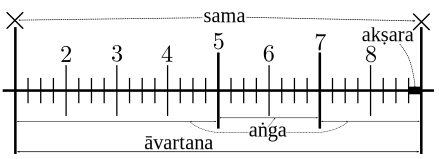
\includegraphics[scale=0.60]{talaFigs/adi_illustrated.pdf}}  \\ 
\subfloat[\Gls{khanda chapu} \gls{tala}]{\label{fig:taala:kchapu} \hspace{0.2cm} \includegraphics[scale=0.60]{talaFigs/kChapu.pdf} \hspace{0.4cm}} %\hspace{0.5cm}
 \subfloat[\Gls{rupaka} \gls{tala}]{\label{fig:taala:rupaka} \includegraphics[scale=0.60]{talaFigs/rupaka.pdf}} %\hspace{0.5cm}
\subfloat[\Gls{mishra chapu} \gls{tala}]{\label{fig:taala:mchapu} \hspace{0.4cm} 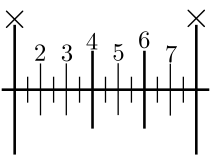
\includegraphics[scale=0.60]{talaFigs/mChapu.pdf}} 
\caption[Four popular Carnatic \glspl{tala}]{An \gls{avartana} of four popular Carnatic \glspl{tala}, showing the \glspl{akshara} (all time ticks), beats (numbered time ticks), \glspl{anga} (long and bold time ticks) and the sama ($\times$). \Gls{adi} \gls{tala} is also illustrated using the terminology used in the dissertation.}\label{fig:taala:carnatic}
\end{figure}

Carnatic music has a sophisticated \gls{tala} system that incorporates the concepts described above. There are seven basic \glspl{tala} defined with different \glspl{anga}, each with five variants leading to the popular 35 \gls{tala} system \cite{samba:98:southMusic}. Each of these 35 \glspl{tala} can be set in five different \gls{nade}, leading to 175 different combinations. However, most of these \glspl{tala} are extremely rare in performances with just over a ten \glspl{tala} that can be regularly seen in concerts. A majority of pieces are composed in four popular \glspl{tala} - \gls{adi}, \gls{rupaka}, \gls{mishra chapu}, and \gls{khanda chapu}. The structure of those four popular \glspl{tala} in Carnatic music are described in \tabref{tab:cm:talastruct} and illustrated in \figref{fig:taala:carnatic}, all in \gls{chaturashra} \gls{nade} (division of a beat into two or four \glspl{akshara}). The different concepts related to the \glspl{tala} of Carnatic music are also illustrated\footnote{Some audio examples illustrating these \glspl{tala} and structure of more \glspl{tala} at \url{http://compmusic.upf.edu/examples-taala-carnatic}} in \figref{fig:taala:adi}. The figure shows the \glspl{akshara} with time-ticks, beats of the cycle with numbered longer time-ticks, and the sama in the cycle using $\times$. The \gls{anga} boundaries are highlighted using bold and long time-ticks e.g. \gls{adi} \gls{tala} has 8 beats in a cycle, with 4 \glspl{akshara} in each beat leading to 32 \glspl{akshara} in a cycle, while \gls{rupaka} \gls{tala} has 12 \glspl{akshara} in a cycle, with 4 \glspl{akshara} in each of its 3 beats. 

The case of non-isochronous beat \glspl{tala}, \gls{mishra chapu} and \gls{khanda chapu}, need a special mention here. \figref{fig:taala:mchapu} shows \gls{mishra chapu} to consist 14 \glspl{akshara} in a cycle. The 14 \glspl{akshara} have a definite unequal grouping structure of 6+4+4 (or 6+8 in some cases) and the boundaries of these groups are shown with visual gestures, and hence form the beats of this \gls{tala} \cite{samba:98:southMusic}. However, in common practice, \gls{mishra chapu} can also be divided into seven equal beats. In this dissertation, we consider \gls{mishra chapu} to consist of seven uniform beats as numbered in \figref{fig:taala:mchapu}, with beats $\times$, 4 and 6 being visually displayed. Similarly, \gls{khanda chapu} has 10 \glspl{akshara} in a cycle grouped into two groups as 4+6. In the scope of this dissertation, \gls{khanda chapu} can be interpreted to consist of 5 equal length beats. In the dissertation, we focus on the most popular \glspl{tala} for analysis, all of which are in caturaśra \gls{nade}. But for completeness, an example of \gls{tishra} \gls{nade}, where each beat is divided into 3 (or 6) \gls{akshara} is illustrated for \gls{adi} \gls{tala} in \figref{fig:taala:aditishra}. We can clearly see that a \gls{tishra} \gls{nade} \gls{adi} \gls{tala} has 8 beats of 3 \glspl{akshara} each, leading to 24 \glspl{akshara} in a cycle. 
\begin{figure}
  \centering
 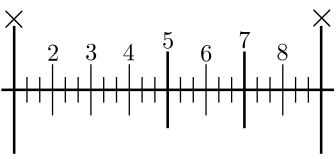
\includegraphics[scale=0.63]{talaFigs/adi_tishra.pdf}
\caption[Structure of \gls{tishra} \gls{nade} \gls{adi} \gls{tala}]{The structure of \gls{tishra} \gls{nade} \gls{adi} \gls{tala}, to contrast with the popularly used \gls{chaturashra} \gls{nade}. Note the three \gls{akshara} beats, and only 24 \gls{akshara} cycle, as compared to the 32 \gls{akshara} cycle in its \gls{chaturashra} \gls{nade} counterpart.}\label{fig:taala:aditishra}
\end{figure}

Most performances of Carnatic music are accompanied by the percussion instrument mridangam (\gls{mridangam}), a double-sided barrel drum. There could however be other percussion accompaniments such as \gls{ghatam} (the clay pot), \gls{khanjira} (the Indian tambourine), thevil (a two sided drum) and \gls{morsing} (the Indian jaw harp), which follow the mridangam closely. All these instruments (except the khañjira) are pitched percussion instruments and are tuned to the tonic\index{Tonic note} of the lead voice. Since the progression through the \gls{tala} cycles is explicitly shown through hand gestures, the mridangam is provided with substantial freedom of rhythmic improvisation during the performance. The \gls{tala} only provides a metrical construct, within which several different rhythmic patterns can be played and improvised.

The solo performed with the percussion accompaniments, called a \gls{tani avartana}, demonstrates the wide variety of rhythms that can be played in a particular \gls{tala}. The solo performance by the percussion ensemble follows the main piece of the concert. The solo is an elaborate rhythmic improvisation within the framework of the \gls{tala}, but with much improvisation on the percussion patterns. The \gls{tani} strives to present a showcase of the \gls{tala} with a variety of percussion and rhythmic patterns that can be played in the tala. The percussion instruments duel and complement each other in a solo of each instrument, with all instruments coming together to a cadential end. The patterns played can last longer than one \gls{avartana}, but stay within the framework of the \gls{tala}. A \gls{tani avartana} is a showcase of the skill and talent of the percussion artists. It is replete with a variety of percussion patterns and hence is very useful for analysis of percussion patterns. The tani is often performed with a subset of the percussion instruments. The mridangam is always present, while the other instruments are optional. 
\begin{table}
\centering
\begin{tabular}{@{}lll@{}}\toprule
ID & Syllable & Description\tabularnewline \midrule
1 & \syl{AC} & A semi ringing stroke on the right head \tabularnewline \addlinespace[2pt]
2 & \syl{ACT} & \syl{AC} with \syl{TH}/\syl{TM}\tabularnewline \addlinespace[2pt]
3 & \syl{CH} & A ringing stroke on the right head\tabularnewline \addlinespace[2pt]
4 & \syl{CHT} & \syl{CH} with \syl{TH}/\syl{TM}\tabularnewline \addlinespace[2pt]
5 & \syl{DM} & A strong ringing stroke on the right head\tabularnewline \addlinespace[2pt]
6 & \syl{DH3} & A closed stroke on the right head (variant-1)\tabularnewline \addlinespace[2pt]
7 & \syl{DH3T} & \syl{DH3} with \syl{TH}\tabularnewline \addlinespace[2pt]
8 & \syl{DH3M} & \syl{DH3} with \syl{TM} \tabularnewline \addlinespace[2pt]
9 & \syl{DH4} & A closed stroke on the right head (variant-2) \tabularnewline \addlinespace[2pt]
10 & \syl{DH4T} & \syl{DH3} with \syl{TH}/\syl{TM}\tabularnewline \addlinespace[2pt]
11 & \syl{DN} & A pitched resonant stroke on the right head \tabularnewline \addlinespace[2pt]
12 & \syl{DNT} & \syl{DN} with \syl{TH}/\syl{TM}\tabularnewline \addlinespace[2pt]
13 & \syl{LF} & Long finger stroke on the right head\tabularnewline \addlinespace[2pt]
14 & \syl{LFT} & \syl{LF} with \syl{TH}/\syl{TM} \tabularnewline \addlinespace[2pt]
15 & \syl{NM} & A sharp pitched stroke on the right head \tabularnewline \addlinespace[2pt]
16 & \syl{NMT} & \syl{NM} with \syl{TH}/\syl{TM} \tabularnewline \addlinespace[2pt]
17 & \syl{TH} & A closed bass stroke on the left head\tabularnewline \addlinespace[2pt]
18 & \syl{TA} & A closed sharp stroke on the right head\tabularnewline \addlinespace[2pt]
19 & \syl{TAT} & \syl{TA} with \syl{TH}/\syl{TM}\tabularnewline \addlinespace[2pt]
20 & \syl{TM} & An open bass stroke on the left head\tabularnewline \addlinespace[2pt]
21 & \syl{TG} & Pitch modulated bass stroke on the left head\tabularnewline \bottomrule
\end{tabular}
\caption[The syllables used in Carnatic music percussion]{The syllables (\glspl{solkattu}) used in mridangam, grouped based on timbre along with the symbol we use for the syllable group in this dissertation. The last column also provides a short description. Most strokes are combinations of left+right strokes on the mridangam.} \label{tab:mridangam:bolmap}
\end{table}

Percussion in Carnatic music is organized and transmitted orally with the use of onomatopoeic\index{Onomatopoeia} oral mnemonic syllables\index{Oral mnemonic syllable} (called \gls{solkattu}) representative of the different strokes of the mridangam. An oral recitation of these syllables is itself an art form called \gls{konnakol}\index{Vocal percussion}, and is often a part of a \gls{tani avartana}. The syllables used belong to mridangam, but is widely used with other percussion instruments used in Carnatic music. These syllables vary across schools, but provide a good representation system to define, describe and discover percussion patterns. We explore the use of these syllables for \gls{MIR} tasks further in the dissertation. 

We consulted a senior professional Carnatic percussionist for the complete set of strokes that can be played with the mridangam. The stroke syllables of the mridangam represent the combined timbre of the left and right drum heads, and hence over 45 different strokes can be played on the mridangam. However, many of the timbrally similar strokes can be grouped together into syllable groups, assuming that such a timbral grouping is sufficient for discovery of timbrally similar percussion patterns. This timbre based grouping further enables us to work with the variability in syllables across different schools. The syllable groups, the symbol we use for them in this dissertation, and a short description is shown in \tabref{tab:mridangam:bolmap}. The different stroke names are not indicated in the table since they vary. For simplicity and brevity, we will refer to the syllable groups as just syllables in this work when there is no ambiguity. Finally however, we carefully note that the syllables also have a loosely defined functional role, and such a timbre based grouping used in the thesis is an approximation done only for computational analysis approaches. 
% 
\subsection[Rhythm and percussion in Hindustani music]{Rhythm and percussion in\\ Hindustani music}
% \dtext{How is rhythm organized. What is lay, taal. Different terms associated with the taal, matras, and then some more terms. Average characteristic of rhythm - tempo ranges, thekas, vibhaags (section/organs), nades, explain the figures. Tabl and its role. Possibility of non-isochorous beats, but our definition of isochronous beats in the thesis and how we can get non-isochronous beats from isochronous ones later on.}
%
%
\begin{table}[t]
\centering
\begin{tabular}{@{}lccr@{}}\toprule
\Gls{taal}  & \# \gls{vibhaag} & \# \glspl{matra} & \gls{matra} grouping \tabularnewline \midrule
\Gls{teental} & 4 & 16 & 4,4,4,4   \tabularnewline
\Gls{ektal} & 6 & 12 & 2,2,2,2,2,2 \tabularnewline
\Gls{jhaptal} & 4 & 10 & 2,3,2,3   \tabularnewline
\Gls{rupak} & 3 & 7 & 3,2,2        \tabularnewline \bottomrule
\end{tabular}
\caption[Structure of Hindustani \glspl{taal}]{Structure of Hindustani \glspl{taal}. For each \gls{taal},the number of \glspl{vibhaag} and the number of \glspl{matra} in each \gls{avart} is shown. The last column of the table shows the grouping of the \glspl{matra} in the \gls{avart} into \glspl{vibhaag}, and the length of each \gls{vibhaag}, e.g. each avart of \gls{rupak} has three \glspl{vibhaag} consisting of three, two, two \glspl{matra} respectively.}\label{tab:hm:taalstruct}
\end{table}
%
\begin{figure}
  \centering
\subfloat[\Gls{teental}, illustrated]{\label{fig:taal:teen} 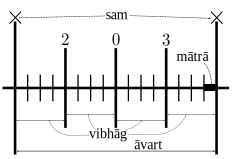
\includegraphics[scale=0.85]{talaFigs/teentaal_illustrated.pdf}} \hspace{0.3cm}
\subfloat[\Gls{rupak}]{\label{fig:taal:rupak} 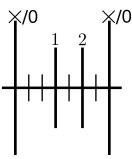
\includegraphics[scale=0.85]{talaFigs/rupaktaal.pdf}}\\
 \subfloat[\Gls{ektal}]{\label{fig:taal:ek} \includegraphics[scale=0.85]{talaFigs/ektaal.pdf}}
 \hspace{1cm}
 \subfloat[\Gls{jhaptal}]{\label{fig:taal:jhap} 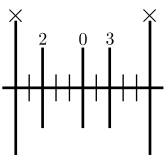
\includegraphics[scale=0.85]{talaFigs/jhaptaal.pdf}}
\caption[Four popular Hindustani \glspl{taal}]{An \gls{avart} of four popular Hindustani \glspl{taal}, showing the \glspl{matra} (all time ticks), \glspl{vibhaag} (long and bold time ticks) and the sam ($\times$). \Gls{teental} is also illustrated using the terminology used in this article.}
\label{fig:taal:hindustani}
\end{figure}
% 
\citeA{clayton:00:time} provides a comprehensive introduction to rhythm in Hindustani music. The definition of \gls{taal} in Hindustani music is similar to the \gls{tala} in Carnatic music. A \gls{taal} has fixed-length cycles, each of which is called an \gls{avart}. An \gls{avart} is divided into isochronous basic time units called \gls{matra}. The \glspl{matra} of a \gls{taal} are grouped into sections, sometimes with unequal time-spans, called the \glspl{vibhaag}. \Glspl{vibhaag} are indicated through the hand gestures of a \gls{thali} (clap) and a \gls{khali} (wave). The first \gls{matra} of an \gls{avart} (the downbeat) is referred to as \gls{sam}, marking the end of the previous cycle and the beginning of the next cycle. The first \gls{matra} of the cycle (\gls{sam}) is highly significant structurally, with many important melodic and rhythmic events happening at the sam. The sam also frequently marks the coming together of the rhythmic streams of soloist and accompanist, and the resolution point for rhythmic tension \cite[p. 81]{clayton:00:time}.

There are also tempo classes called \gls{lay} in Hindustani music which can vary between ati-vilaṁbit (very slow), \gls{vilambit} (slow), \gls{madhyam} (medium), \gls{dhrut} (fast) to ati-dhr̥t (very fast). Depending on the \gls{lay}, the \gls{matra} may be further subdivided into shorter time-span pulsations, indicated through additional filler strokes of the \gls{tabla}. However, since these pulses are not well defined in music theory, we consider \gls{matra} to be lowest level pulse in the scope of this dissertation.

As with Carnatic music, even in Hindustani music, there are significant differences to the terminology describing meter in Eurogenetic music. The definition of beat pulsation, as foot tapping instances in time, is also a problem with Hindustani music. Depending on the lay, the \gls{matra} can be defined to be the subdivisions (for \gls{dhrut} lay) or as beats (for \gls{vilambit} and \gls{madhyam} \gls{lay}). To maintain consistency, using accepted conventions, we note that the concepts of \gls{matra} and the \gls{avart} of Hindustani music bear analogy to the beat and the bar metrical levels of Eurogenetic music. This implies that there is no well defined subdivision pulsation defined in Hindustani music. The possibly unequal \glspl{vibhaag} are the sections of the \gls{taal}.
%
\begin{figure}
  \centering
 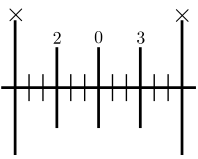
\includegraphics[scale=0.85]{talaFigs/ektaal_drut.pdf}
\caption[\Gls{ektal} in \gls{dhrut} \gls{lay}]{An alternative structure of \Gls{ektal} in \gls{dhrut} \gls{lay}}\label{fig:taal:drutektal}
\end{figure}

There are over 70 different Hindustani \glspl{taal} defined, while about 15 \glspl{taal} are performed in practice. \figref{fig:taal:hindustani} shows four popular Hindustani \glspl{taal} - \gls{teental}, \gls{ektal}, \gls{jhaptal}, and \gls{rupak}. The structure of these \glspl{taal} are also described in \tabref{tab:hm:taalstruct}. The figure also shows the \gls{sam} (shown as $ \times $) and the \glspl{vibhaag} ( indicated with \gls{thali}/\gls{khali} pattern using numerals). A \gls{khali} is shown with a $0$, while the \gls{thali} are shown with non-zero numerals. The \gls{thali} and \gls{khali} pattern of a \gls{taal} decides the accents of the \gls{taal}. The \gls{sam} has the strongest accent (with certain exceptions, such as \gls{rupak}) followed by the \gls{thali} instants. The \gls{khali} instants have the least accent. 
\begin{table}[t]
\centering
\tabcolsep=0.10cm
\begin{tabular}{@{}lp{2.7cm}cp{6cm}@{}}
\toprule
ID & \centering\Glspl{bol} & Symbol & \centering Description\tabularnewline \midrule
1 & D, DA, DAA  & \syl{DA} & A closed stroke on the \gls{dayan} (right drum) \tabularnewline \addlinespace[2pt]
2 & N, NA, TAA & \syl{NA} & A ringing stroke on the \gls{dayan} \tabularnewline \addlinespace[2pt]
3 & DI, DIN, DING & \syl{DIN} & An open stroke on the \gls{dayan} \tabularnewline \addlinespace[2pt]
4 & KA, KAT, KE, KI, KII & \syl{KI} & A closed stroke on the \gls{bayan} (left drum)\tabularnewline \addlinespace[2pt] 
5 & GA, GHE, GE, GHI, GI & \syl{GE} & A modulated stroke on the left drum\tabularnewline \addlinespace[2pt]
6 & KDA, KRA, KRI, KRU & \syl{KDA} & Two quick successive strokes (played as a flam), one each on \gls{dayan} and \gls{bayan}\tabularnewline \addlinespace[2pt]
7 & TA, TI, RA  & \syl{TA} & A closed stroke on the \gls{dayan}\tabularnewline \addlinespace[2pt]
8 & CHAP, TIT & \syl{TIT} & A closed stroke on the \gls{dayan} \tabularnewline \addlinespace[2pt]
9 & DHA & \syl{DHA} & A resonant combined stroke with \syl{NA} and \syl{GE}\tabularnewline \addlinespace[2pt]
10 & DHE & \syl{DHE} & A closed combined stroke played with the full palm on the \gls{dayan} with a closed \syl{GE}\tabularnewline \bottomrule
\end{tabular}
\caption[The \gls{tabla} \glspl{bol} used in Hindustani music]{(1/2) The \glspl{bol} used in \gls{tabla} are shown in the second column, grouped by similarity of timbre. The symbol we use for the syllable group in the dissertation is shown in the third column and a short description of the timbre \cite{beronja:08:tabla} is shown in the fourth column. Combined stroke has strokes on left and right drum played together simultaneously (\textbf{contd...}).}\label{tab:tabla:bolmap}
\end{table}%Skipped: KAR, GHEN, TUN - not in dataset. The symbols \syl{DHA}, \syl{DHE}, \syl{DHET}, \syl{DHI}, \syl{DHIN}, \syl{RE}, \syl{TE}, \syl{TII}, \syl{TIN}, \syl{TRA} have a one to one mapping with a syllable of the same name and hence not shown in the table. We compile a comprehensive set of syllables in tabla.
%
\begin{table}[t]
\centering
\tabcolsep=0.10cm
\addtocounter{table}{-1}  % hack
\begin{tabular}{@{}lP{2.7cm}cp{6cm}@{}}
\toprule
ID & \centering\Glspl{bol} & Symbol & \centering Description\tabularnewline \midrule
11 & DHET & \syl{DHET} & A combined stroke played with a closed stroke on \gls{dayan} with \syl{GE}\tabularnewline \addlinespace[2pt]
12 & DHI & \syl{DHI} & A closed combined stroke with \syl{GE} and a soft resonant stroke on \gls{dayan} \tabularnewline \addlinespace[2pt]
13 & DHIN & \syl{DHIN} & An open combined stroke with \syl{GE} and a soft resonant stroke on \gls{dayan} \tabularnewline \addlinespace[2pt]
14 & RE & \syl{RE} & A closed stroke on the \gls{dayan} played with the palm\tabularnewline \addlinespace[2pt]
15 & TE & \syl{TE} & A closed stroke on the \gls{dayan} played with the palm\tabularnewline \addlinespace[2pt]
16 & TII & \syl{TII} & A combined stroke with \syl{KI} and a soft closed resonant stroke on \gls{dayan}\tabularnewline \addlinespace[2pt]
17 & TIN & \syl{TIN} & A combined stroke with \syl{KI} and a soft open resonant stroke on \gls{dayan}\tabularnewline \addlinespace[2pt]
18 & TRA & \syl{TRA} & Two quick successive closed strokes on \gls{dayan} (played as a flam)\tabularnewline \bottomrule
\end{tabular}
\caption[]{(2/2) The \glspl{bol} used in \gls{tabla} are shown in second column, grouped by similarity of timbre. The symbol we use for the syllable group in the dissertation is shown in the third column and a short description of the timbre \cite{beronja:08:tabla} is shown in the fourth column. Combined stroke has strokes on left and right drum played together simultaneously.}
\end{table}
%

A \gls{jhaptal} \gls{avart} has 10 \glspl{matra} with four unequal \glspl{vibhaag} (\figref{fig:taal:jhap}), while a \gls{teental} \gls{avart} has 16 \glspl{matra} with four equal \glspl{vibhaag} (\figref{fig:taal:teen}). We can also note from \figref{fig:taal:rupak} that the \gls{sam} is a khāli in \gls{rupak}, which has 7 \glspl{matra} with three unequal \glspl{vibhaag}. 
%

The special case of \gls{ektal} needs additional mention here. \Gls{ektal} has six equal duration \glspl{vibhaag} and 12 \glspl{matra} in a cycle as shown in \figref{fig:taal:ek}. However, in \gls{dhrut} \gls{lay}, an alternative structure emerges, which is represented as four equal duration \glspl{vibhaag} of three \glspl{matra} each as shown in \figref{fig:taal:drutektal}. For consistency, we use the structure as shown in \figref{fig:taal:ek} in this dissertation. 

Hindustani music uses the \gls{tabla} as the main percussion accompaniment. It consists of two drums: a left hand bass drum called the \gls{bayan} or \gls{digga} and a right hand drum called the \gls{dayan} that can produce a variety of pitched sounds. Similar to mridangam, the \gls{tabla} repertoire is transmitted using onomatopoeic\index{Onomatopoeia} oral mnemonic syllables\index{Oral mnemonic syllable} called the \gls{bol}. 

Similar to lead melody in Hindustani music, \gls{tabla} has different stylistic schools called \glspl{gharana}. The repertoires of major \glspl{gharana} of \gls{tabla} differ in aspects such as the use of specific \glspl{bol}, the dynamics of strokes, ornamentation and rhythmical phrases~\cite[p.~60]{beronja:08:tabla}. But there are also many similarities due to the fact that the same forms and standard phrases reappear across these repertoires \cite[p.~52]{gottlieb:93:tabla}. 

The \glspl{bol} of the \gls{tabla} vary marginally within and across \glspl{gharana}, and several \glspl{bol} can represent the same stroke on the \gls{tabla}. To address this issue, we grouped the full set of 38 syllables into timbrally similar groups resulting into a reduced set of 18 syllable groups as shown in \tabref{tab:tabla:bolmap}. Though each syllable on its own has a functional role, this timbral grouping is presumed to be sufficient for discovery of percussion patterns. For the remainder of the dissertation, we limit ourselves to the reduced set of syllable groups and use them to represent patterns. For convenience, when it is clear from the context, we call the syllable groups as just syllables and denote them by the symbols in \tabref{tab:tabla:bolmap}. A brief description of the timbre is also provided for each syllable. 
\begin{table}
  \centering
\subfloat[\Gls{teental}]{\label{fig:theka:teen} 
\begin{tabular}{cccc|cccc}
\toprule
$\times$ &  &  &  & \textbf{2} &  &  &  \tabularnewline 
$\times$ & 2 & 3 & 4 & 5 & 6 & 7 & 8 \tabularnewline
\syl{DHA} & \syl{DHIN} & \syl{DHIN} & \syl{DHA} & \syl{DHA} & \syl{DHIN} & \syl{DHIN} & \syl{DHA} \tabularnewline \midrule 
\textbf{0} &  &  &  & \textbf{3} &  &  &  \tabularnewline 
9 & 10 & 11 & 12 & 13 & 14 & 15 & 16 \tabularnewline
\syl{DHA} & \syl{TIN} & \syl{TIN} & \syl{NA} & \syl{NA} & \syl{DHIN} & \syl{DHIN} & \syl{DHA} \tabularnewline \bottomrule
\end{tabular}}\\
%
\subfloat[\Gls{ektal}]{\label{fig:theka:ek} 
\begin{tabular}{cc|cc|cc}
\toprule
$\times$ &  & \textbf{0} &  & \textbf{2} &  \tabularnewline
$\times$ & 2 & 3 & 4 & 5 & 6 \tabularnewline
\syl{DHIN} & \syl{DHIN} & \syl{DHA GE} & \syl{TIRAKITA}  & \syl{TUN} & \syl{NA} \tabularnewline \midrule
\textbf{0} &  & \textbf{3} & & \textbf{4} &  \tabularnewline
7 & 8 & 9 & 10 & 11 & 12 \tabularnewline
\syl{KAT} & \syl{TA} & \syl{DHA GE} & \syl{TIRAKITA}  & \syl{DHIN} & \syl{NA} \tabularnewline \bottomrule
\end{tabular}}\\
%
\subfloat[\Gls{jhaptal}]{\label{fig:theka:jhap} 
\begin{tabular}{cc|ccc|cc|ccc}
\toprule
$\times$ &  & \textbf{2} & & & \textbf{0} &  & \textbf{3} & & \tabularnewline
$\times$ & 2 & 3 & 4 & 5 & 6 & 7 & 8 & 9 & 10 \tabularnewline
\syl{DHI} & \syl{NA} & \syl{DHI} & \syl{DHI}  & \syl{NA} & \syl{TI} & \syl{NA} & \syl{DHI} & \syl{DHI} & \syl{NA} \tabularnewline \bottomrule
\end{tabular}}\\
%
\subfloat[\Gls{rupak}]{\label{fig:theka:rupak} 
\begin{tabular}{ccc|cc|cc}
\toprule
$\times$\textbf{/0} &  & & \textbf{1} & & \textbf{2} & \tabularnewline
$\times$ & 2 & 3 & 4 & 5 & 6 & 7 \tabularnewline
\syl{TIN} & \syl{TIN} & \syl{NA} & \syl{DHI}  & \syl{NA} & \syl{DHI} & \syl{NA} \tabularnewline \bottomrule
\end{tabular}}\\
%
\caption[The \glspl{theka} for popular Hindustani \glspl{taal}]{The \glspl{theka} for four popular Hindustani \glspl{taal}, showing the \gls{bol} for each \gls{matra}. The \gls{sam} is shown with $\protect\times$ and \glspl{vibhaag} boundaries are separated with a vertical line. Each \gls{matra} of a cycle has equal duration.}\label{fig:theka:hindustani}
\end{table}

\Gls{tabla} acts as the timekeeper during the performance indicating the progression through the \gls{taal} cycles using pre-defined rhythmic patterns (called the \gls{theka}) for each \gls{taal}. The lead musician improvises over these cycles, with limited rhythmic improvisation during the main piece. The \glspl{theka} are specific canonical \gls{tabla} \gls{bol} patterns defined for each \gls{taal} as illustrated in \tabref{fig:theka:hindustani}. However, the musician playing \gls{tabla} improvises these patterns playing many variations with filler strokes and short improvisatory patterns. \citeA{miron:11:thesis}, \citeA{clayton:00:time}, \citeA{dutta:95:tabla}, \citeA{beronja:08:tabla}, and \citeA{naimpalli:05:tabla} provide a more detailed discussion of \gls{taal} in Hindustani music including \glspl{theka} for commonly used \glspl{taal}\footnote{Some audio examples illustrating the \glspl{taal} and structure of more \glspl{taal} at \url{http://compmusic.upf.edu/examples-taal-hindustani}}. 

To showcase the nuances of a \gls{taal} as well as the skill of the percussionist with the \gls{tabla}, Hindustani music performances feature \gls{tabla} solos. A \gls{tabla} solo is intricate and elaborate, with a variety of pre-composed forms used for developing further elaborations. There are specific principles that govern these elaborations~\cite[p.~42]{gottlieb:93:tabla}. Musical forms of \gls{tabla} such as the \gls{theka}, \gls{kayda}, \gls{palta}, \gls{rela}, \gls{peshkar} and \gls{gat} are a part of the solo performance and have different functional and aesthetic roles in a solo performance. A percussion solo shows a variety of improvisation possible in the framework of the \gls{taal}, with the role of timekeeping taken up by the lead musician during the solo. 

In Hindustani music, the tempo is measured in \glspl{matra} per minute (\mpm). The music has a wide range of tempo, divided into tempo classes called \gls{lay} as described before. The mainly performed ones are the the slow (\gls{vilambit}), medium (\gls{madhyam}), and fast (\gls{dhrut}) classes. The boundary between these tempo classes is not well defined with possible overlaps. In this dissertation, after consultation with a professional Hindustani musician, we use the commonly agreed tempo ranges for these classes: \gls{vilambit} \gls{lay} for a median tempo between 10-60 \mpm, \gls{madhyam} \gls{lay} for 60-150 \mpm, and \gls{dhrut} \gls{lay} for $>$150 \mpm. This large range of allowed tempi means that the duration of a \gls{taal} cycle in Hindustani music ranges from less than 2 seconds to over a minute. A \gls{matra} in \gls{vilambit} \gls{lay} hence can last about 6 seconds, and to maintain a continuous rhythmic pulse, several filler strokes are played on the \gls{tabla}. Hence the surface rhythm apparent from audio recordings can be quite different from the underlying metrical structure.
%
\subsection[Carnatic and Hindustani music: Comparison]{Carnatic and Hindustani music:\\ A comparison}
We compare and contrast some of the rhythm related concepts in Carnatic and Hindustani music, so that it can be used for better comparison of \gls{MIR} approaches for these musics. 

Both the music traditions are oral traditions, with a lot of allowed scope for improvisation. Even a fixed composition is interpreted with significant freedom by the musicians, as long as they adhere to the framework of the \gls{raga} and \gls{tala}. The concept of cyclical metrical structures is shared by both music cultures, while the components of the \gls{tala} are less similar. The first pulse of the cycle is important in both cultures and has significant melodic and rhythmic events. The sections of the \gls{tala} cycle need not be equal in duration. The \gls{tala} does not change over single piece (with rare exceptions), but since Hindustani music recordings are distributed as full concerts, there is a possible change of piece in the middle of a recording, with a change of \gls{taal} and/or \gls{lay}. 

Neither of the music cultures use a metronome during performance, which means that the responsibility of maintaining a regular pulse rests with the musicians. This leads to a flexible time-varying nature of tempo, with most often the tempo increasing (and the piece getting ``faster") with time. The range of tempo in Hindustani music is large (from 10 \mpm\ to over 350 \mpm), while Carnatic music is performed in a smaller range of tempo. This has the implication that while \gls{taal} cycles can be quite long in Hindustani music, while Carnatic music \gls{tala} cycles are shorter (often shorter than 15 second). 

In Hindustani and Carnatic music, the percussion accompaniments \gls{tabla} and mridangam are tuned to the tonic of the lead musician. Both these instruments are capable of producing a rich variety of timbres. The playing style depends on the composition or the lead melody being rendered, and both are improvised during performance. Both have specific \glspl{theka} for the exposition of the \gls{tala}, though \glspl{theka} are a little more flexibly defined in Carnatic Music. Both \gls{tabla} and mridangam have their own set of onomatopoeic\index{Onomatopoeia} mnemonic oral syllables that provide a language for percussion, which even have evolved into art forms of reciting these syllables in a performance. Representing percussion patterns with these syllables is musically well-defined and an accurate representation of those patterns. 

The surface rhythm in both the music cultures provide cues to the underlying \gls{tala} structures. In Hindustani music, \gls{tabla} is a very important cue to the underlying \gls{taal} progression. All \glspl{taal} have a definite accent and \gls{tabla} stroke pattern defined by the \gls{theka} which is mostly followed except in improvisatory passages. The surface rhythm consists of these accents and specific strokes, but is also replete with other strokes, fillers and expressive additions. Filler strokes are employed in slow pieces with long cycles. In Carnatic music, as discussed earlier, the progression through the \gls{tala} is shown through visual gestures and hence there is no need for definitive cues in the surface rhythm. However, the percussion phrases played on the mridangam, the melodic phrases and the lyrics of the composition provide cues to the underlying \gls{tala}. Unlike \gls{tabla} strokes, mridangam strokes are less indicative of the current position in the cycle of a \gls{tala}. 

Unmetered forms of music exist in both the music cultures. The most important unmetered form in Hindustani music is the \gls{alap} and in Carnatic music is the \gls{alapana}, both of which are melodic improvisational forms based on a \gls{raga}. An understanding of the rhythmic behavior of unmetered forms is far from trivial for musicologists and even practicing musicians \cite{clayton:96:freerhythm}. \citeA{widdess:94:dhrupad} presented an interesting discussion of the notion of pulsation in \glspl{alap} and a disagreement about it among performers. For this reason, we believe that rhythmic analysis of unmetered forms should be reserved for a study more from a musicological perspective and hence we do not consider it in this dissertation. 
% \comment{Sufficient for now. Add more here as appropriate later on}
%
%
%\dtext{Talk about similarities in structure of taalas and in percussion patterns and hence how lot of algorithms can make use of this similarity.}
%\dtext{Language and tranliteration used in the thesis correspond to Kannada and when clear, we use \gls{tala} to mean both \gls{tala} and \gls{taal}}. 
%
%\subsection{Rhythm in Turkish music} %\comment{In less detail ...}
%\dtext{In Turkish music, rhythm is organized around usuls. Usuls have a left and right pattern, they can be very long as well.}
\subsection{Percussion in Beijing opera}\label{sec:bkgnd:bopercussion}
% \dtext{Beijing opera is a test case to test out percussion patterns. Similar to Indian music an hence an introductory study can be done on this as well. Instruments used, how they sound, how are patterns formed, how is it similar to Indian music.}
The main focus of this dissertation is Indian art music, however, within the context of CompMusic, there are other music cultures that share similar music concepts and hence are suitable candidates for test and extend our approaches to those musics. Beijing opera is one such music culture that shares the concept of a syllabic percussion\index{Syllabic percussion} system, similar to Indian art music. However, the syllabic percussion system in Beijing opera is simpler and more well defined than Indian art music, and hence is a test case to validate our approaches to percussion pattern transcription and discovery. A basic introduction to percussion in Beijing opera is provided, since some of our approaches to percussion pattern analysis are first tested on Beijing opera and then extended to Indian art music. 

Beijing opera (\Gls{jingju}, \gls{cn:jingju}), also called Peking opera,\index{Beijing opera} is one of the most representative genres of Chinese traditional performing arts, integrating theatrical acting with singing and instrumental accompaniment. It is an active art form and exists in the current social and cultural contexts, with a large audience and significant musicological literature. One of the main characteristics of Beijing opera aesthetics is the remarkable rhythmicity that governs the acting overall. From the stylized recitatives to the performers' movements on stage and the sequence of scenes, every element presented is integrated into an overall rhythmic flow. The main element that keeps this rhythmicity is the percussion ensemble, and the main means to fulfil this task is a set of predefined and labeled percussion patterns. 

The percussion ensemble in \gls{jingju} establishes and maintains the rhythm in a performance and guides the progression of sections in an aria. Firstly, the percussion provides a base to indicate the rhythmic modes, called the \textit{banshi}, and accompanies the singing voice. Secondly, the percussion ensemble plays different kinds of predefined, fixed, labeled patterns that create a context for different parts of the aria. They signal important structural points in the play. A performance starts and ends with percussion patterns, they generally introduce and conclude arias, and mark transition points within them. They accompany the actors' movements on stage and set the mood of the play, the scene, the aria or a section of the aria. 
%
\begin{table}
\centering
\begin{tabular}{p{5cm}|p{3.5cm}|c}
\toprule 
\centering \textbf{Syllables} & \centering \textbf{Instruments} & \textbf{Symbol} \tabularnewline \midrule 
\gls{ba1} (\gls{cn:ba1},~\gls{cn:ba2}),  \gls{ben} (\gls{cn:ben}), \gls{da1} (\gls{cn:da1}), \gls{da2} (\gls{cn:da2}), \gls{dong1} (\gls{cn:dong1},~\gls{cn:dong2}), \gls{duo} (\gls{cn:duo}), \gls{long} (\gls{cn:long}), \gls{yi} (\gls{cn:yi}) & \centering \gls{bangu} & \syl{DA} \tabularnewline \hline 
\gls{lai} (\gls{cn:lai}), \gls{tai} (\gls{cn:tai}), \gls{ling} (\gls{cn:ling}) & \centering \gls{xiaoluo} & \syl{TAI} \tabularnewline \hline 
\gls{qi} (\gls{cn:qi}), \gls{pu} (\gls{cn:pu}) & \centering \gls{naobo} & \syl{QI}\tabularnewline \hline 
\gls{qie} (\gls{cn:qie}) & \centering \gls{naobo}+\gls{xiaoluo} & \syl{QIE} \tabularnewline \hline 
\gls{cang} (\gls{cn:cang}), \gls{kuang} (\gls{cn:kuang}),
\gls{kong} (\gls{cn:kong})  & \centering \gls{daluo} + $<$\gls{naobo}$>$ + $<$\gls{xiaoluo}$>$& \syl{CANG} \tabularnewline \bottomrule
\end{tabular}
\caption[Syllables used in Beijing opera (\gls{jingju}) percussion]{Syllables used in Beijing opera percussion and their grouping used in this dissertation. Column 2 shows the instrument combination used to produce the syllable, with the instrument shown between $< >$ being optional. Column 3 shows the symbol used for the syllable group in this dissertation.}\label{tab:bo:sylmap}
\end{table}

The percussion patterns in \gls{jingju} music can be defined as sequences of strokes played by different combinations of the percussion instruments, and the resulting variety of timbres are transmitted using oral syllables as mnemonics\index{Oral mnemonic syllable}. The percussion ensemble is formed mainly by five instruments played by four musicians. The \textit{ban} (a wooden clapper) and the \textit{danpigu} (a wooden drum struck by two wooden sticks) are played by one single performer, and are therefore known by a conjoint name, \gls{bangu} (clapper-drum). The other three instruments are idiophones\index{Idiophone}: the \gls{xiaoluo} (small gong), the \gls{daluo} (big gong) and the \gls{naobo} (cymbals) \cite{lee:99:chineseInst,wichmann:91:BOaural}. 
\begin{figure}
\centering
\subfloat[][\gls{daobantou} \gls{cn:daobantou}]{\label{fig:bopatt:daobantou}\includegraphics[width=\textwidth]{jingjuPatts/DaobanTou.pdf}} \\
\subfloat[][\gls{manchangchui} \gls{cn:manchangchui}]{\label{fig:bopatt:manchangchui}\includegraphics[width=\textwidth]{jingjuPatts/ManChangchui.pdf}} \\
\subfloat[][\gls{duotou} \gls{cn:duotou}]{\label{fig:bopatt:duotou}\includegraphics[width=\textwidth]{jingjuPatts/Duotou.pdf}} \\
\caption[Percussion patterns in Beijing opera (\gls{jingju})]{(1/2) Scores for percussion patterns in \gls{jingju}, showing the instruments and a syllabic representation of the pattern using the unmapped syllables, and the mapped syllable groups shown in \tabref{tab:bo:sylmap} (\textbf{contd...})}\label{fig:bopatt:scores}
\end{figure}
%
\begin{figure}
\addtocounter{subfigure}{3} % hack 
\addtocounter{figure}{-1}  % hack
\centering
\subfloat[][\gls{xiaoduotou} \gls{cn:xiaoduotou}]{\label{fig:bopatt:xiaoduotou}\includegraphics[width=\textwidth]{jingjuPatts/XiaoluoDuotou.pdf}} \\
\subfloat[][\gls{shanchui} \gls{cn:shanchui}]{\label{fig:bopatt:shanchui}\includegraphics[width=\textwidth]{jingjuPatts/Shanchui.pdf}} \\
\caption[]{(2/2) Scores for percussion patterns in \gls{jingju}, showing the instruments and a syllabic representation of the pattern using the unmapped syllables, and the mapped syllable groups shown in \tabref{tab:bo:sylmap}}%\label{fig:bopatterns}
\end{figure}

\textit{Bangu} has a high pitched drum-like sound while the rest of three instruments are metallophones with distinct timbres\footnote{A few annotated audio examples of these instruments can be found at \url{http://compmusic.upf.edu/examples-percussion-bo}}. Each of the different sounds that these instruments can produce individually, either through different playing techniques or through different dynamics, as well as the sounds that are produced by a combination of different instruments have an associated syllable that represent them \cite{wenyi:07:boperf}. In \gls{jingju}, several syllables can be mapped to a single timbre. This many-syllable to one-timbre mapping is useful to reduce the syllable space for computational analysis of percussion patterns. 

We first mapped each syllable to one or several of the instrument categories considered for analysis, as explained by \citeA{tian:14:icassp}, without considering differences in playing technique or dynamics. Based on inputs from expert musicologists, we then grouped the syllables with similar timbres into five syllable groups - \syl{DA}, \syl{TAI}, \syl{QI}, \syl{QIE}, and \syl{CANG}, as shown in \tabref{tab:bo:sylmap}. Every individual stroke of the \gls{bangu}, both drum and clappers, have been grouped as \syl{DA}. In the rest of the syllable groups, the \gls{bangu} can be played simultaneously or not. The single strokes of the \gls{xiaoluo} and the \gls{naobo} are called \syl{TAI} and \syl{QI} respectively, and the combined stroke of these two instruments together is the syllable \syl{QIE}. Finally, any stroke of the \gls{daluo} or any combination that includes \gls{daluo} has been notated as \syl{CANG}. This mapping to a reduced set of syllable groups is only for the purpose of computational analysis. For the remainder of the dissertation, we limit ourselves to the reduced set of syllable groups and use them to represent the patterns. For convenience, when it is clear from the context, we call the syllable groups as just syllables, and denote them by the common symbol in column 3 of \tabref{tab:bo:sylmap}. Hence, in the current task, there are five syllable groups.

Each percussion pattern is a sequence of syllables in their pre-established order, along with their specific rhythmic structure and dynamic features. A particular feature of the oral syllabic system for Beijing opera percussion that makes it especially interesting is that the syllables that form a pattern refer to the ensemble as a whole, and not to particular instruments. Each particular pattern thus has a single unique syllabic representation shared by all the performers. 

In practice, there is a library of limited set of named patterns (called \gls{pattern}, \gls{cn:pattern}) that are played in a performance, with each of these having a specific role in the arias. Although a definite agreed number for the total number of these patterns is lacking, some estimations, e.g. by \citeA{wenyi:07:boperf}, suggest the existence of around ninety of them. \figref{fig:bopatt:scores} shows the scores for five predominantly used percussion patterns in \gls{jingju} - \gls{daobantou}, \gls{manchangchui}, \gls{duotou}, \gls{xiaoduotou}, and \gls{shanchui}\footnote{These pattern scores are also listed at \url{http://compmusic.upf.edu/bo-perc-patterns}}. The figure also shows how a possible transcription in staff notation, adapted from the scores provided by \citeA{wenyi:07:boperf}, can be simplified in a single line by the oral syllabic system. Hence, the use of these oral syllabic sequences simplify and unify the representation of these patterns played by an ensemble. 

Since one of the main functions of the patterns is to accompany the movements of actors on stage, the overall length and the relative duration of each stroke can vary notably, which makes it difficult to set a stable pulse or a definite meter. The time signature and the measure bars used in \figref{fig:bopatt:scores}, as suggested by \citeA{wenyi:07:boperf}, are only indicative and fail to convey the rhythmic flexibility of the pattern. Furthermore, many patterns (such as \gls{shanchui} shown in \figref{fig:bopatt:shanchui}) accompany scenic movements of undefined duration. In these cases, certain syllable subsequences in the pattern are repeated indefinitely, e.g. the subsequence \gls{cang}-\gls{tai}-\gls{qie}-\gls{tai} in \gls{shanchui} can be repeated indefinitely until the scene completes.  

From this brief introduction, it can be seen that there are similarities between the percussion systems in \gls{jingju} and Indian art music. Being simpler, \gls{jingju} can be used a test case for approaches to percussion pattern transcription and discovery in syllabic percussion systems, a topic that is explored further in the dissertation. We focus only on the aural dimension of Beijing opera. For convenience, we use the term Beijing opera to refer to the music in Beijing opera, ignoring the theatrical aspect in it.  
%
\section[A review of automatic rhythm analysis]{A review of automatic rhythm\\ analysis}
%\note{This is the state of the art for the most common tasks that will be explored. Indian music specific state of the art and evaluation will be explored in next chapter.}
\begin{figure}
\centering
\includegraphics[height=0.9\textwidth,angle=90]{blockDiags/rhythmDescUnits.png}
\caption[Functional units of a rhythm description system]{Functional units of a rhythm description system as described by \protect\citeA{gouyon:05:phdthesis} (Figure reproduced with permission)}\label{fig:sota:rhythmdescsys}
\end{figure}
Automatic rhythm analysis has been an important research area within \gls{MIR}, with over a decade of research on several relevant rhythm and percussion related problems. A review of the state of the art of the relevant rhythm research problems is presented to provide a basis for further work proposed in the dissertation. The review of previous works in this section is generic and not specific to Indian art music. A more detailed review of approaches specific to Indian art music, and an evaluation of the state of the art on Indian art music is discussed in \chapref{chap:probdef}. 
%\comment{For each of the below methods, specify broad methods, and the specific approaches, explaining the state of the art methods in a paragraph each. Put down figures if needed, to explain better the methods.}
%
%\subsection{Rhythm description}
%\note{Reproduced from the Fabien's thesis - the old approach. What it is missing in our context needs to be explained later on.}

Several researchers have suggested a decomposition of automatic rhythm description into complementary modules, each considering a specific task, and possibly using information and outputs from other modules~\cite{gouyon:05:phdthesis,gouyon:05:review}. An example of such a rhythm description system is shown in \figref{fig:sota:rhythmdescsys}. Starting from audio and/or music scores, the system shows several rhythm analysis modules that give out important rhythm analysis outputs such as tempo, beats, swing, time signature, and rhythmic patterns. Though such a rhythm description for Indian art music would involve significant changes, this system nevertheless provides a suitable basic framework to start formulating research problems. 
\subsection{Onset detection}\label{sec:bkgnd:onsetdetect}
%\note{Figure about onset characteristics in a spectrogram}
Musical note/stroke onset detection\index{Onset detection} is the most fundamental pre-processing task for most rhythm analysis problems. Within the task of onset detection, we can include the task of extracting features from audio that are indicative of onsets, and the approaches to obtain the onsets from those features. 

A musical note/stroke onset\index{Onset} is defined as the single instant that marks a detectable start of an extended transient of the note/stroke, when the music audio signal evolves quickly in a non-trivial manner over a short time \cite{bello:05:onset}. In simpler words, onsets mark the start of a melodic note or a percussion stroke. Onsets mark important musical events in time and the automatic detection of onset events is an essential part of many music signal analysis algorithms. Onset detection has various applications in identification, retrieval, musicological analysis, audio editing and coding, content-based processing and many other applications.
 
A detailed tutorial on onset detection methods is provided by \citeA{bello:05:onset}, with additional improvements suggested by \citeA{dixon:06:onset}. Onset detection needs transient detection in audio signals. The transients can be measured either in amplitude, energy, phase, frequency, and several other signal parameters. Most approaches to onset detection involve a signal pre-processing step, followed by a signal reduction (extracting features that are indicative of transients) into an onset detection function, and a peak-picking step that estimates the onset times as the peaks on the onset detection function. 

The pre-processing step is optional and aims to enhance relevant parts of the signal. Signal reduction often involves frame-wise \gls{STFT} based analysis of signals, often in multiple frequency bands using filter banks to capture frequency information from different instruments in the audio signal. The result of such a feature extraction is an onset detection function, also sometimes called a novelty function\index{Novelty function}. The peaks of the onset detection function are then the onsets. 

There are several methods to compute the onset detection function, based on signal features and probabilistic models. The signal features include time domain features such as amplitude envelope, that works well for percussive onsets. More popular features are spectral features that measure some form change in spectral amplitudes and energy. The spectral flux\index{Spectral flux} feature is the most often used one, which measures a positive change (for onsets, negative change would indicate offsets) of spectral energy across frames of audio. The spectral flux can be computed both with the magnitude of \gls{STFT} or the complex \gls{STFT}, across adjacent frames or across a local set of frames. There are several ways a spectral flux can be computed, described by \citeA{bello:05:onset}, and further improved by many researchers, e.g. as LogFilt-SpecFlux by \citeA{bock:12:onseteval}. 

The definition of an onset could become ambiguous in the case of instruments having longer transient times without sharp bursts of energy rises. \citeA{vos:81:perception} approached this issue by introducing the concept of perceptual onset as the time when the most salient metrical feature of the music signal is perceived relative to its physical onset. \citeA{dixon:06:onset} examined and proposed improvements to the then state of the art spectral methods. \citeA{klapuri:99:onset} proposed a method utilizing band-wise processing and a psychoacoustic model of intensity coding to detect perceptual onsets.
\subsubsection{Instrument-wise onset detection}
Instrument-wise onset detection refers to detecting the onsets of specific instruments from an audio signal that is a mixture of many music instruments. By detecting onsets of specific instruments, we can focus on characterizing the aspect of music that the instrument dominates, e.g. the onsets of the percussion instruments might be more useful for rhythmic analysis. One approach to instrument-wise onset detection is to separate out the part of audio that contains the information from the specific instrument we wish to extract onsets from. To detect percussion onsets, it might be advantageous to enhance the percussive parts of the signal and suppress the harmonic component. 

\gls{HPSS} aims to separate an audio signal into harmonic (melodic instruments) and percussive (drums) components. Though an accurate source separation for human listening is a difficult task, \gls{HPSS} for further computational analysis is simpler. Most approaches to \gls{HPSS} process the spectrogram using characteristics shown by melodic and percussive music sources. The basic idea is that melodic sources show up as horizontal lines (owing to all their harmonics) in the spectrogram while percussive sources (due to their sharp attacks and broadband spectra) as vertical lines~\cite{fitzgerald:10:hpss}. This enables us to enhance the vertical spectral lines (or suppress the horizontal spectral lines) to enhance the percussive component of the audio, and vice versa to enhance the melodic component, such as the approaches by \citeA{thoshkahna:11:hpss} and \citeA{ono:08:hpss}. 

A more informed approach uses a predominant melody extraction algorithm, which tracks the fundamental frequency\index{Fundamental frequency} (\fzero) of the audio signal to uses signal analysis tools to suppress all the harmonics of the melodic source. The residual left in the spectrogram corresponds to the percussive component of the signal. The Harmonic plus residual model by \citeA{serra:89:phdthesis} along with a melody extraction algorithm e.g. by \citeA{salamon:12:melody} are some of the tools that could be used for the task. The onsets from the percussion enhanced signal would give us the percussion onsets. 
%\dtext{Juan's paper. Onset detection, and features for Onset detection also to be described here. Enhanced onset detection, pool aggregation of onsets. Spectral flux, superflux, and some signal examples.}
% Talk about spectral flux and super flux. 
%\subsection{Instrument identification}
%\note{Write about instrument identification and tracking from mixtures - NMF and other methods. In brief.}
\subsection{Tempo estimation}\label{sec:bkgnd:tempoest}
% \note{Old methods, Fabien Gouyon. Autocorrelation, tempogram as a feature, etc. And some newer approaches, and how tempo is often a byproduct in tasks.}
Tempo\index{Tempo tracking} estimation refers to estimating the period of the predominant pulse in the music recording, at the correct metrical level of the beat (or at a different metrical level, if musically well defined). The definition of such a tempo is not clear and there can be disagreement on the correct metrical level. Further, in pieces where tempo can change over time, it is necessary to estimate a time varying tempo curve through the piece instead of single tempo estimate for a music piece. Despite the metrical ambiguity, tempo estimation is a useful task for further analysis tasks such as beat and meter tracking. 

Tempo estimation algorithms use some form of periodicity estimation using mid-level features extracted from audio, mostly the onset detection functions. An autocorrelation of such a novelty function is a basic measure of periodicity. Following the onset detection functions, there are distinctly two different approaches that have been used for tempo induction. Some methods, such as the BeatRoot system proposed by \citeA{dixon:07:beatroot} are pulse selection methods that measure the \gls{IOI} and use them to estimate the tempo. An \gls{IOI} histogram has peaks at the periodicity of the beat period, which can then be measured. However, significant metrical ambiguity exists in such approaches since the \gls{IOI} histograms are often multimodal. The other approaches, such as the ones by \citeA{klapuri:06:meter,davies:07:beat,ellis:07:beat} derive a periodicity function from the detection function, which provides an estimate of tempo. 

Several mid-level audio features have been proposed to estimate a time varying tempo curve: a few examples of such features include novelty functions\index{Novelty function} used for structural segmentation~\cite{foote:00:novelty}, Tempogram
~\cite{grosche:11:tempogram}\index{Tempogram} and Predominant Local Pulse~\cite{grosche:11:pulse}. % Recent approaches use methods that estimate within the framework of meter or beat tracking. 
% 
% \update{add more later}
\subsection{Beat tracking}\label{sec:bkgnd:beattrack}
% \note{Old methods, described from Jose'e thesis. Klapuri\cite{klapuri:06:meter}, Davies\cite{davies:07:beat}, Peeters papers. How its an ill defined task, and there can ambiguities. McKinney's work and evaluation. Some datasets available for the task.} 
In the context of \gls{MIR}, beat tracking\index{Beat tracking} is commonly defined as determining the time instances in the audio recording where a human listener is likely to tap his/her foot to the music. Being an important and relevant \gls{MIR} task, several approaches have been proposed for beat tracking on audio music recordings in a wide variety of genres. Conventional beat tracking algorithms generally use three main sub components - feature extraction, tempo induction, and beat induction. The rhythm features extracted are typically based on onsets and onset detection functions. A good overview of several beat tracking algorithms is provided by \citeA{holzapfel:12:beat}. 

\citeA{dixon:07:beatroot} uses a multiple agent architecture using a collection of tempo hypotheses, which are all tested for continuity to obtain the set of beat locations. \citeA{ellis:07:beat} developed a beat tracking algorithm based on dynamic programming, which computes a global set of optimal beat candidates, given an accent signal and a tempo estimate. The algorithm pursues a tradeoff between the temporal continuity of beats and the salience of the detection function using the dynamic programming approach. The main drawback of the algorithm is the assumption of a constant tempo, which causes problems for music with varying tempo. Further, errors in tempo estimation translate to an incorrect estimation of the beats. \citeA{wu:11:beatDP} also proposed a similar dynamic programming approach to beat tracking, but with extensions to handle a time-varying tempo. \citeA{davies:07:beat} proposed a context dependent beat tracking algorithm which handles varying tempo, by providing a two state model in which the first state tracks the tempo changes and provides continuity, while the second state tracks the beat pulses maintaining contextual continuity, assuming a constant tempo. 

The algorithm proposed by \citeA{klapuri:06:meter} estimates the musical meter jointly at three metrical levels of bar, beat and subdivision, which are referred to as measure, tactus and tatum, respectively. A time frequency analysis computes accent signals in four frequency bands, which are aimed at emphasizing changes due to note onsets in the signal. A bank of comb filter resonators is applied for periodicity analysis to each of the four accent signals. The periodicities thus found are processed by a probabilistic model that incorporates musical knowledge to perform a joint estimation of the tatum, tactus, and measure pulsations. \citeA{peeters:11:beat} present another approach for simultaneous beat and downbeat tracking using a probabilistic framework using beat templates built using linear discriminant analysis and an algorithm that estimates the beat positions within a bar, with an evaluation on six different datasets. Some early approaches have explored particle filtering and approximate inference for beat tracking task \cite{hainsworth:03:pfbeat}, while probabilistic graphical models (see \secref{sec:bkgnd:pgm}) have also been explored for the task of beat tracking~\cite{lang:04:thesis,lang:05:beat}. 

\citeA{bock:11:nnbeat} proposed a data driven approach to beat tracking using context-aware neural networks. A \gls{RNN} with \gls{LSTM} cells~\cite{hochreiter:97:lstm} can learn contextual information and can classify and predict time series when there are long time lags of unknown size between important events. Mel-spectrogram based spectral features and their relative differences were used to train a bidirectional \gls{LSTM} network to perform a frame by frame beat classification of a signal. The network outputs a beat activation function directly using the input signal and an autocorrelation function was then used to determine the predominant tempo to eliminate the erroneously detected beats and complement the missing beats. Recently, neural network beat trackers have significantly improved beat tracking state of the art and have aimed towards joint beat and downbeat tracking. 

Ensemble approaches have also been proposed for beat tracking, which uses mutual agreement between several beat trackers to improve beat tracking performance~\cite{holzapfel:12:beat}. The approach is useful to identify pieces that are difficult for beat tracking, and also to create a dataset of such difficult pieces. The disagreement between beat trackers indicates that a piece is difficult to track (for the automatic beat trackers) and hence such pieces can further be used to improve beat tracking performance with better beat trackers. 

Beat tracking is an important \gls{MIR} task and has been a part of \gls{MIREX} challenge since its inception. There are also several datasets that have been used for evaluating beat tracking algorithms, such as the SMC dataset \cite{holzapfel:12:beat}, Ballroom dataset \cite{gouyon:06:tempo,dixon:04:pattern,bock:11:nnbeat}, RWC database \cite{goto:06:rwc}, Hainsworth dataset \cite{hainsworth:03:pfbeat}, McKinney dataset \cite{moelants:04:tempo}, and more recently, the GTZAN-Rhythm dataset \cite{marchand:15:gtzanrhythm} that adds the beat, downbeat and swing annotations to the GTZAN dataset \cite{tzanetakis:02:genre}. We use the Ballroom dataset to evaluate our approaches in this dissertation. 

Despite a significant effort, beat tracking algorithms still need to be significantly improved for use in practical systems. They suffer from metrical level ambiguities and poor generalizability to other musical genres. The beats are assumed to be isochronous, which is another limitation of the beat tracking algorithms so far. However, several improvements have been suggested to improve the performance. \citeA{zapata:13:beatVS} explore the use of voice suppression to improve beat tracking performance. A mutual agreement of several beat trackers can also be used to assign a confidence level to the beat tracking performance and identify samples difficult for beat tracking~\cite{holzapfel:12:beat,zapata:12:beat}. 
\subsection{Time signature estimation}
Automatic rhythm annotation problems apart from onset detection, beat and tempo tracking have been less explored by the MIR community. \citeA{gainza:09:meter} used beat tracking to perform musical meter detection for western music using a beat similarity matrix based approach and \citeA{foote:01:beatSpec} suggested a new beat spectrum for rhythm analysis. \citeA{uhle:03:tempo} extended the tempo tracking framework for time signature and micro-time estimation on percussive music. 

In the method proposed by \citeA{pikrakis:04:meter}, time signature is estimated from a self-distance matrix computed from \gls{MFCC} extracted from the audio signal. To this end, minima in the distance matrix are assumed to be caused by repetitions related to the metrical structure of the piece. Hence, this algorithm does not track pulsations in a piece, but relies on existence of patterns caused by general repetitions in the \gls{MFCC} features. Because \gls{MFCC} features capture timbral characteristics, it can be stated that similarities in local timbre are used by the algorithm. The algorithm was tested on East-European music styles, including Greek traditional dance music.
%
\subsection{Downbeat tracking}
% \note{Relatively new, some old approaches do exist. Hockman et al\cite{hockman:12:downbeat}, Simon and Juan's work included.}
Downbeat tracking\index{Downbeat tracking} is the estimation of the instant of beginning of the bar. The methods described in this section were developed for the identification of downbeats within sequences of beats. So far mainly music with a $4/4$ time signature has been the focus of evaluations, usually in the form of collections of Eurogenetic popular and/or classical music. 

The approach presented by \citeA{davies:06:downbeat} is based on the assumption that percussive events and harmonic changes tend to be correlated with the downbeat position. Therefore, they partition an audio signal into beat segments and compute a \gls{STFT} of each segment, neglecting frequencies above 1.4 kHz. Then the magnitude differences between all neighboring blocks are computed. Subsequently, for a given bar length in beats, the sequence of bar length distant segments that is related to the maximum spectral change is chosen as downbeats. 

\citeA{hockman:12:downbeat} presented an algorithm for detecting downbeats in music signals, specifically at hardcore, jungle, and drum and bass genres of music. Their approach combines information from low level onset event information, periodicity information from beat tracking, and high-level information from a regression model trained with classic breakbeats. The approach is an extension of a downbeat detection system proposed by \citeA{jehan:05:phdthesis} that applies support vector regression. The features of the regression consist of Mel-frequency spectral coefficients, loudness descriptors, and chroma features, all computed for the separate beat segments. The extension proposed by \citeauthor{hockman:12:downbeat} comprises a post-processing of the regression, a combination with a low-frequency onset detection, and a beat-time weighting. While the post-processing compensates for spurious downbeat detections, the combination of the regression with a low-frequency onset feature is motivated by the fact that strong bass drums tend to be located at the downbeat for the form of music they considered.

Downbeat estimation has been addressed as a part of beat tracking \cite{klapuri:06:meter,peeters:11:beat} resulting in a joint estimation of beats and downbeats. In both cases, a probabilistic framework is used to estimate the downbeats from the beats.
%
\subsection{Meter tracking}\label{sec:bkgnd:mt}
Most of the approaches presented so far considered the task of beat tracking and downbeat tracking as separate tasks. The task of estimating the tempo, beats and the downbeats is what we refer to as meter tracking\index{Meter tracking}. Recent approaches in meter tracking have successfully applied Bayesian models that jointly estimate beat and downbeats together, using rhythmic patterns learned from onset detection functions as features~\cite{krebs:13:bpm,bock:14:multimodel,krebs:15:pf}. Recent interest has also been to explore deep neural networks for meter tracking, where multiple musically inspired features capturing different aspects of music have been used~\cite{durand:15:dbtrack}, with extensions that used feature adapted convolutional neural networks~\cite{durand:16:feature}. 
%\comment{To be completed: Write about downbeat tracking with neural networks. Work of Bock, Simon and Juan Bello}. 
%\comment{Elaborate more here on recent Bayesian methods and those using deep learning for the task.}
% \dtext{Meter Inference = rhythm class + tempo + beat + downbeat tracking, Meter Tracking = Tempo + beat + downbeat tracking}
% We want to do all together. Some recent Bayesian methods and those using deep learning for the task. Using rhythmic patterns to jointly track all metrical levels. 
\subsection{Evaluation measures}\label{sec:bkgnd:evalmeas}
% Precision, Recall, f-Measure, infoGain, CMLt, CMLc, AMLt, AMLc, p-Score. 
There are several measures that have been proposed for measuring the accuracy of performance of beat and downbeat trackers \cite{davies:09:beatEval}. Starting with an annotated dataset with beat marked audio, these measures consider the accuracy of beat locations estimated, continuity of beats, and the metrical level at which the beats were tracked. There have also been information theoretic measures proposed based on the entropy of beat tracking errors, which measures the extent of correlation between the annotations and the estimated beat locations. \citeA{mckinney:07:beatEval} present a survey of the performance of several beat tracking algorithms using multiple accuracy measures\footnote{An implementation of the evaluation measures is available at \url{http://code.soundsoftware.ac.uk/projects/beat-evaluation/}}. For our evaluation, we use the f-measure, information gain, $\cmlt$ and $\amlt$ measures. These measures are characterized by a set of diverse properties and are often used in beat tracking evaluations in \gls{MIREX}\footnote{e.g. MIREX 2012, \url{http://www.music-ir.org/mirex/wiki/2012:Audio\_Beat\_Tracking}}. The measures are now explained for the task of beat tracking, but extend to downbeat tracking as well, with the same tolerances.

For a music piece, given the ground truth beat times and the estimated beat sequence, a beat is marked as correctly detected if it lies inside a tolerance window around a ground truth annotation. The f-measure (denoted as $\fmeas$ in this dissertation) is a number between $0$ and $1$ computed as the harmonic mean of the popular information retrieval performance metrics - \textit{precision} and \textit{recall}. Precision ($\precision$) is the ratio between the number of correctly detected beats and all detected beats, while recall ($\recall$) is the ratio between the number of correctly detected beats and the total annotated beats. The f-measure can take a maximum value of 1, while beats tapped on the off-beat relative to annotations will be assigned an f-measure of 0. Estimated beats with time-spans either half or double the annotated time-span are penalized with a value of 0.667.

The $\cmlt$ measure (Correct Metrical Levels, no continuity) is a number between 0 and 1, is the ratio between the number of correctly estimated beats divided by the number of annotated beats. It takes the value of 1 only for sequences that coincide with the annotations. It does not penalize discontinuities in beat tracking as the CML$_\mathrm{c}$ (Correct Metrical Levels, continuity required) measure, but penalizes any beats tracked at half or double time-spans of the annotated metrical level. $\amlt$ (Allowed Metrical Levels with no continuity required) is also a number between $0$ and $1$, where beat sequences are considered as correct if the beats occur on the off-beat, or are double or half of the annotated tempo, allowing for metrical ambiguities. The value of this measure is then the ratio between the number of correctly estimated beats divided by the number of annotated beats. Similar to f-measure, small misalignments in the estimated beats are allowed by applying tolerance windows before computing the $\cmlt$ and $\amlt$ measures.

Information gain ($\infoGain$) aims at determining if there exists any kind of relation between the estimated beats and the annotations, and indicates how much information the estimated beats provide about the annotations. It uses the entropy of the beat error distribution and can be interpreted as an information theoretic measure. This measure is a numerical score that takes a value of 0 bits only for completely unrelated sequences and by using the default setting of 40 bins in the beat error histogram, a maximum value of 5.3 bits for highly related beat sequences. Timing errors are calculated between an annotation and all beat estimations within a one-beat length window around the annotation. Then, a beat error histogram is formed from the resulting timing error sequence. A numerical score is derived by measuring the K-L divergence between the observed error histogram and the uniform distribution. 
\subsection{Rhythm similarity measures}\label{sec:bkgnd:rhythmsim}
Defining and extracting music similarity is one of the primary areas of \gls{MIR}. An important component of defining overall similarity between two music pieces is rhythmic similarity. Similarity measures to compare rhythms have been explored both with audio and symbolic scores. These rhythm similarity measures are quite useful in computational musicology to compare rhythms. 

Rhythm similarity\index{Rhythm similarity} measures have been used to classify and compare rhythms, trace ancestry of rhythms using phylogenetic analyses, to match prototypical rhythm patterns to their micro-variations. \citeA{toussaint:04:similarity} discusses several measures and compares them based on how much insight they provide about the inter-relationships that exist among families of rhythm. 

One approach to compare rhythmic content of music is by using onset patterns (OP)\index{Onset patterns}, as initially presented by \citeA{pohle:09:rhythmSim}. Starting from a magnitude spectrum obtained from the \gls{STFT} of a monophonic piece of music, a set of energy coefficients are computed in 32 logarithmically spaced frequency bands. A band-wise accent signal is then derived by applying a moving average filter and half wave rectification to each of the 32 bands. A second \gls{STFT} operating on longer time scale (8 second window with 1 second hop) is applied to each band-wise accent signal. This way, a description of periodicities referred to as OP features~\cite{holzapfel:11:RhythmSimSMC} is obtained for 5 bands per octave, and 5 periodicity octaves from 30 \bpm\ to 960 \bpm. The rhythm of a whole sample is described by the mean of the OP obtained from the various segments of this sample. \citeA{pohle:09:rhythmSim} showed that combining rhythmic descriptors with a timbral component improved the performance of the task of rhythm similarity computation on the ``Ballroom Dancers" collection (Ballroom dataset). 

\citeA{holzapfel:10:scale} use the scale transform to compute rhythm descriptors to classify Greek traditional dances and Turkish traditional songs. The first step is a computation of an accent signal. To this end, the sum of the 32 band-wise accent signals used for the OP features are applied to obtain a single vector describing the note onset characteristics. Then, within the moving windows of eight seconds length, autocorrelation coefficients are computed from this accent signal and then transformed into the scale domain by applying a discrete Scale Transform. For one piece, the mean of the Scale Transform Magnitudes (STM) obtained from all the analysis windows are the STM descriptors of the rhythmic content of the piece. Both the mapping onto a logarithmic axis of the magnitudes in the second \gls{STFT} in the OP features, and the application of a Scale transform in the STM features provide varying degrees of robustness to tempo changes. \citeA{holzapfel:10:scale} provide more details and the exact computation of parameters of the two descriptors. The scale transform is also shown to capture relevant properties of \emph{usuls} (metrical framework in Turkish makam music) and has been used for classifying symbolic traditional Turkish music scores to their \emph{usuls} \cite{holzapfel:09:TurkRhythmSim}. \citeA{holzapfel:11:RhythmSimSMC} discuss improved descriptors for rhythm similarity. 

\citeA{fouloulis:10:similarity} present a system containing two artificial neural networks in cascade - a self-organizing neural network (called SARDNET) and a Multi-Layer Perceptron - that receives a sequence of temporal intervals (performed rhythm pattern) as input and maps it into a given set of prototypical rhythm patterns showing strong evidence that this type of network architecture may be successful to compute similarity between a prototypical rhythm pattern and its micro-variations. \citeA{parry:03:similarity} proposed a similarity metric based on rhythmic elaboration that matches rhythms that share the same beats regardless of tempo or identicalness. Rhythmic elaborations can help an application decide where to transition between songs.
\subsection{Domain-specific approaches}
Including domain specific music knowledge to build culture-aware algorithms is an important focus of the dissertation. From the extracted low level audio features, we can use domain specific prior knowledge to derive mid-level representations. As mentioned earlier, a few examples of such mid-level representations include novelty functions used for structural segmentation~\cite{foote:00:novelty}, Tempogram\index{Tempogram} and Predominant Local Pulse~\cite{grosche:11:tempogram}. Though these functions are not generally built using domain specific parameters, we can easily extend them to incorporate priors based on the music culture, e.g. the kernel size in Novelty computation. 

There are several machine learning algorithms that can include domain specific priors into their modeling parameters. Most probabilistic graphical models\index{Graphical model} allow for including some form of priors and encode complex relationships. Simple examples of these include the kinds of priors and relationships that can be encoded using a \gls{HMM}. Hidden semi-Markov models allow us to encode explicit timing information into the algorithm, which might be very useful for tracking rhythmic events, as explored with some promise for chord recognition by \citeA{chen:12:dhmm}. \gls{DBN} \cite{murphy:02:thesis} based models have been successfully applied for beat and downbeat tracking, and hold significant promise. Context-aware neural networks, as discussed in \secref{sec:bkgnd:beattrack}, might also be useful to bring the modeling capabilities of neural networks to modeling structured data such as music. 
\subsection{Percussion pattern analysis}\label{sec:bkgnd:sotapercpatt}
% \dtext{Some current approaches to transcription, their idea of transcribing instruments. Beatboxing, Klapuri's HMM, drum sequence work by Matthias Mauch.}
%%%%%%%%%%%%%%%%%%%%%%%%
One of the main percussion pattern \index{Percussion pattern}analysis tasks is percussion transcription from audio. Music transcription addresses the analysis of an acoustic musical signal so as to write down the pitch, onset time, duration, and source of each sound that occurs within it \cite{klapuri:06:transcription}. Percussion transcription focuses on percussion and aims to transcribe an audio recording, typically a percussion solo, into a sequence of symbolic drum stroke indicators. Though promising results have been achieved in percussion transcription \cite{gillet:04:drumloops,paulus:05:drum,paulus:06:percTranscription}, state of the art music transcription systems are still clearly inferior to skilled human annotation in their accuracy. 

Most works on music transcription have focused on melodies of pitched instruments. However, recent years have witnessed a growing interest for transcribing non-pitched percussive instruments. The percussion instruments investigated in automatic transcription tasks fall into two main categories: membranophones\index{Membranophone}, such as drums that have a stretched membrane or skin, and idiophones\index{Idiophone}, such as cymbals that produce sound from their own bodies \cite{fletcher:98:physics}. 

To address the problem of percussion transcription, some event-based systems \cite{gillet:04:drumloops,gouyon:02:pulse,goto:94:soundSep,gillet:08:transcription} have been proposed that segment the input signal into events informed by the percussion and then extract and classify features from these segments to uncover its musically meaningful content, such as onsets. An alternative to this approach is to rely on source separation based methods to decompose the input audio signal into basis functions that capture the overall spectral characteristics of the sources. Commonly used source separation techniques and tools such as independent component analysis (ICA) and \gls{NMF} have proven to be useful in percussion onset detection tasks, especially when analyzing mixtures of different percussion instruments \cite{paulus:05:drum,smaragdis:04:convNMF,smaragdis:04:techreportNMF, abdallah:03:probability}. 

A parallel to natural language can be drawn with percussion or drum patterns - patterns composed using a small alphabet can be analogous to words. A corpus-wide analysis of rhythm patterns using a data-driven natural language processing approach was presented by \citeA{mauch:12:patterns}, identifying the analogy between rhythm patterns and natural language. 

\citeA{nakano:04:voicePerc} explored drum pattern retrieval using vocal percussion\index{Vocal percussion}, using an \gls{HMM} based approach. They used onomatopoeia\index{Onomatopoeia} as the internal representation for drum patterns, with a focus on retrieving known fixed sequences from a library of drum patterns with snare and bass drums. \citeA{kapur:04:beatbox} explored query by beatboxing\index{Beatboxing}, aiming to map the beatboxing sounds into the corresponding drum sounds. A distinction to be noted here is that in vocal percussion systems such as beatboxing, the vocalizations form the music itself, and not a means for transmission, which is the case with oral syllables of Indian art music percussion. 

More recently, \citeA{paulus:09:hmmdrum} have proposed the use of connected \glspl{HMM} for drum transcription in polyphonic music. \citeA{thompson:14:transcription} explored the task of drum transcription by classifying bar length rhythm patterns, utilizing low level timbre features and long term statistics from rhythm patterns. Both these approaches aim to transcribe individual drums and not overall timbres due to combinations, and no reference to syllabic percussion is made. However all these approaches have indirectly and implicitly used some form of symbolic representations for drum patterns. % \citeA{tsunoo:11:perc} demonstrated a music classification task using K-means clustering of bar-long percussive patterns and bass lines extracted using one-pass dynamic programming. 
\section{Relevant technical concepts}\label{sec:bkgnd:techconcepts} % Write this section at the very very end
The thesis uses several well established and well studied signal processing and machine learning algorithms and techniques to address automatic rhythm analysis problems. There are excellent resources available to study and understand those models and approaches in depth, and hence only a brief mention of those methods along with references to the resources are provided in this section. The purpose is to list the algorithms and techniques and provide adequate references for a background study, and hence the section is not comprehensive in description. 
\subsection{Bayesian models}\label{sec:bkgnd:pgm}
A probabilistic graphical model\index{Graphical model} is a probabilistic model that expresses conditional dependence between random variables using a graph. A Bayesian model (or a Bayesian network)\index{Bayesian model} is a probabilistic graphical model that represents a set of random variables along and their (conditional) dependencies with a directed acyclic graph. Graphical models are generic models and most of the classical multivariate probabilistic systems (e.g. mixture models, \glspl{HMM} and Kalman filters) are special cases of graphical models. 

With a fundamental dependence on time, any model that aims to accurately represent rhythm and metrical structures should work on sequential data from audio features, and must be able to incorporate several different variables within one probabilistic framework. A \acrfull{DBN} \cite{murphy:02:thesis} is well suited in such cases, since it relates variables over time through conditional (in)dependence relations. A \gls{DBN} is a generalization of the traditional linear state-space models such as Kalman filters and stochastic models such as the \gls{HMM} and provides a general probabilistic representation and inference schemes for arbitrary non-linear and non-gaussian time-dependent processes. 

\glspl{DBN} hence provide an effective and explicit way to encode dependence relationships between different components of rhythm in music and are further explored for meter analysis. The \gls{HMM} is a special case of a \gls{DBN} and is used for modeling percussion syllables in the thesis. The book by \citeA{koller:09:pgm} is a comprehensive guide for probabilistic graphical models including practical applications. \glspl{HMM} have been extensively used in machine learning research, and basics of an \gls{HMM} along with the core problems are discussed in a beginner friendly tutorial by \citeA{rabiner:89:tutorial}. A comprehensive resource to understand and apply \glspl{DBN} in theory and to practical applications is written by \citeA{murphy:02:thesis}.
% \dtext{Bayesian Networks, Markov networks, specific cases of Naive Bayes, HMMs, DBNs, and architectures.}
\subsubsection{Inference in Bayesian models}
Inference with a built Bayesian model refers to the operation in which we estimate the probability distribution of one or more unknown variables (or attributes), given that we know the values of other variables. In the context of rhythm analysis, inference can refer to using the ``observed" audio features extracted from music to estimate the unknown rhythm and meter related variables. 

Exact inference in Bayesian models, in its simplest form involves marginalizing over variables to obtain the distribution over the required set of variables, achieved by direct marginalization, factoring, variable elimination and other techniques~\cite{ambrosio:99:bninf}. With the exception of some toy examples, exact inference is complex, without closed form solutions for real world Bayesian models and hence we resort to approximate methods. 

There are efficient inference algorithms for specific inference problems in \gls{HMM}, one such being the Viterbi algorithm~\cite{rabiner:89:tutorial} to decode the most likely sequence of hidden states given an observed feature sequence. In more complex \glspl{DBN}, \gls{SMC} methods are often effective. \gls{SMC} methods (also called particle filters\index{Particle filter}) are a class of approximate inference algorithms that have been effectively applied for estimating posterior densities in \glspl{DBN}. Particle filters are used for efficient approximate inference in Bayesian models and are described in detail in the tutorial by \citeA{doucet:09:tutorial}. %for meter analysis and
% \dtext{Exact inference, Viterbi algorithm}
%\subsubsection{Sequential Monte Carlo and Sampling methods}
%\dtext{Approximate Monte Carlo methods. Particle filtering, the idea and basics. MPF and AMPF described later on, within the context of Meter tracking in Chapter 5.}
\subsection{Speech recognition technologies and tools}
Automatic speech recognition\index{Speech recognition} aims to build tools and techniques for automatic understanding of speech, primarily focusing on transcribing spoken utterances into written words. Being an important \gls{ICT} for natural language processing, it has received attention from a large research community over the past many decades and has evolved into a mature research area with state of the art methods for the task~\cite{huang:10:sroverview}. While research continues in speech recognition on several open problems, there is a potential to utilize some of its proven technologies and extend them to analogous tasks in \gls{MIR}. There is extensive literature on speech recognition, with comprehensive description provided by, e.g. \citeA{huang:90:hmm}, \citeA{rabiner:93:asr} and recently by \citeA{huang:10:sroverview}. Percussion syllables provide a language for percussion, with a significant analogy to speech. Hence, we explore the use of speech recognition tools for percussion pattern transcription and discovery. 

Percussion transcription follows the standard data flow of speech recognition, aiming to transcribe an audio recording into a sequence of syllables. A string search on transcribed sequence can then be used to search for patterns, using string search methods. However, transcription is often inaccurate with many errors, and any pattern search on transcribed data needs to use approximate search algorithms~\cite{navarro:01:strDist}. There are several other attempts to deal with search in symbolic sequences, many are described in detail by \citeA{typke:05:survey}. Well explored techniques formulate pattern search as \gls{LCS} problem. However, \gls{LCS} does not consider the local correlation while searching for a subsequence~\cite{lin:11:rlcs}. To overcome this limitation, \citeA{lin:11:rlcs} proposed a novel \gls{RLCS} method for music matching, that we adapt for the problem of approximate string search in the thesis. 
%
%\note{A short summary of the chapter to be added here} ?
%
%\subsubsection*{Approximate String Matching}
%\dtext{Write about tools and methods for speech recognition, how to use them, and where they will be useful in this task. Evaluation measures in speech technologies.}
%\dtext{Probably move this to approx string matching section} 
%\begin{figure}
%\centering
%% \captionsetup[subfigure]{labelformat=empty}
%\begin{subfigure}[]{\textwidth}\includegraphics[width=\textwidth]{jingjuPatts/DaobanTou.pdf}
%\caption[\gls{daobantou}]{\gls{daobantou}}\label{fig:bopatt:daobantou}\end{subfigure}
%\vspace{3em}
%\begin{subfigure}[]{\textwidth}\includegraphics[width=\textwidth]{jingjuPatts/ManChangchui.pdf}
%\caption[\gls{manchangchui}]{\gls{manchangchui}}\label{fig:bopatt:manchangchui}\end{subfigure}
%\vspace{3em}
%\begin{subfigure}[]{\textwidth}\includegraphics[width=\textwidth]{jingjuPatts/Duotou.pdf}
%\caption[\gls{duotou}]{\gls{duotou}}\label{fig:bopatt:duotou}\end{subfigure}
%\caption{Percussion patterns in \gls{jingju}}\label{fig:bopatterns}
%\end{figure}
%%
%\begin{figure}
%\ContinuedFloat
%\centering
%\begin{subfigure}[]{\textwidth}\includegraphics[width=\textwidth]{jingjuPatts/XiaoluoDuotou.pdf}
%\caption[\gls{xiaoduotou}]{\gls{xiaoduotou}}\label{fig:bopatt:xiaoduotou}\end{subfigure}
%\vspace{3em}
%\begin{subfigure}[]{\textwidth}\includegraphics[width=\textwidth]{jingjuPatts/Shanchui.pdf}
%\caption[\gls{shanchui}]{\gls{shanchui}}\label{fig:bopatt:shanchui}\end{subfigure}
%
%\caption[]{Percussion patterns in \gls{jingju} (contd...)}\label{fig:bopatterns}
%\end{figure}
%
%
%
%\begin{figure}[ht]
%%\captionsetup[subfigure]{labelformat=empty}
%\begin{center}
%\begin{subfigure}[]{6cm}\includegraphics[scale=1]{dstats/HMDf-teen-IAI.pdf}
%\caption{\Gls{teental}}\label{fig:dstats:HMDf:IAI:teen}\end{subfigure}
%%\hspace{0.1cm}
%\begin{subfigure}[]{6cm}\includegraphics[scale=1]{dstats/HMDf-ek-IAI.pdf}
%\caption{\Gls{ektal}}\label{fig:dstats:HMDf:IAI:teen}\end{subfigure}\\
%\begin{subfigure}[]{6cm}\includegraphics[scale=1]{dstats/HMDf-jhap-IAI.pdf}
%\caption{\Gls{jhaptal}}\label{fig:dstats:HMDf:IAI:teen}\end{subfigure}
%%\hspace{0.1cm}
%\begin{subfigure}[]{6cm}\includegraphics[scale=1]{dstats/HMDf-rupak-IAI.pdf}
%\caption{\Gls{rupak}}\label{fig:dstats:HMDf:IAI:teen}\end{subfigure}
%
%\end{center}
%\end{figure}
%